\begin{figure}[b!]
    \centering
    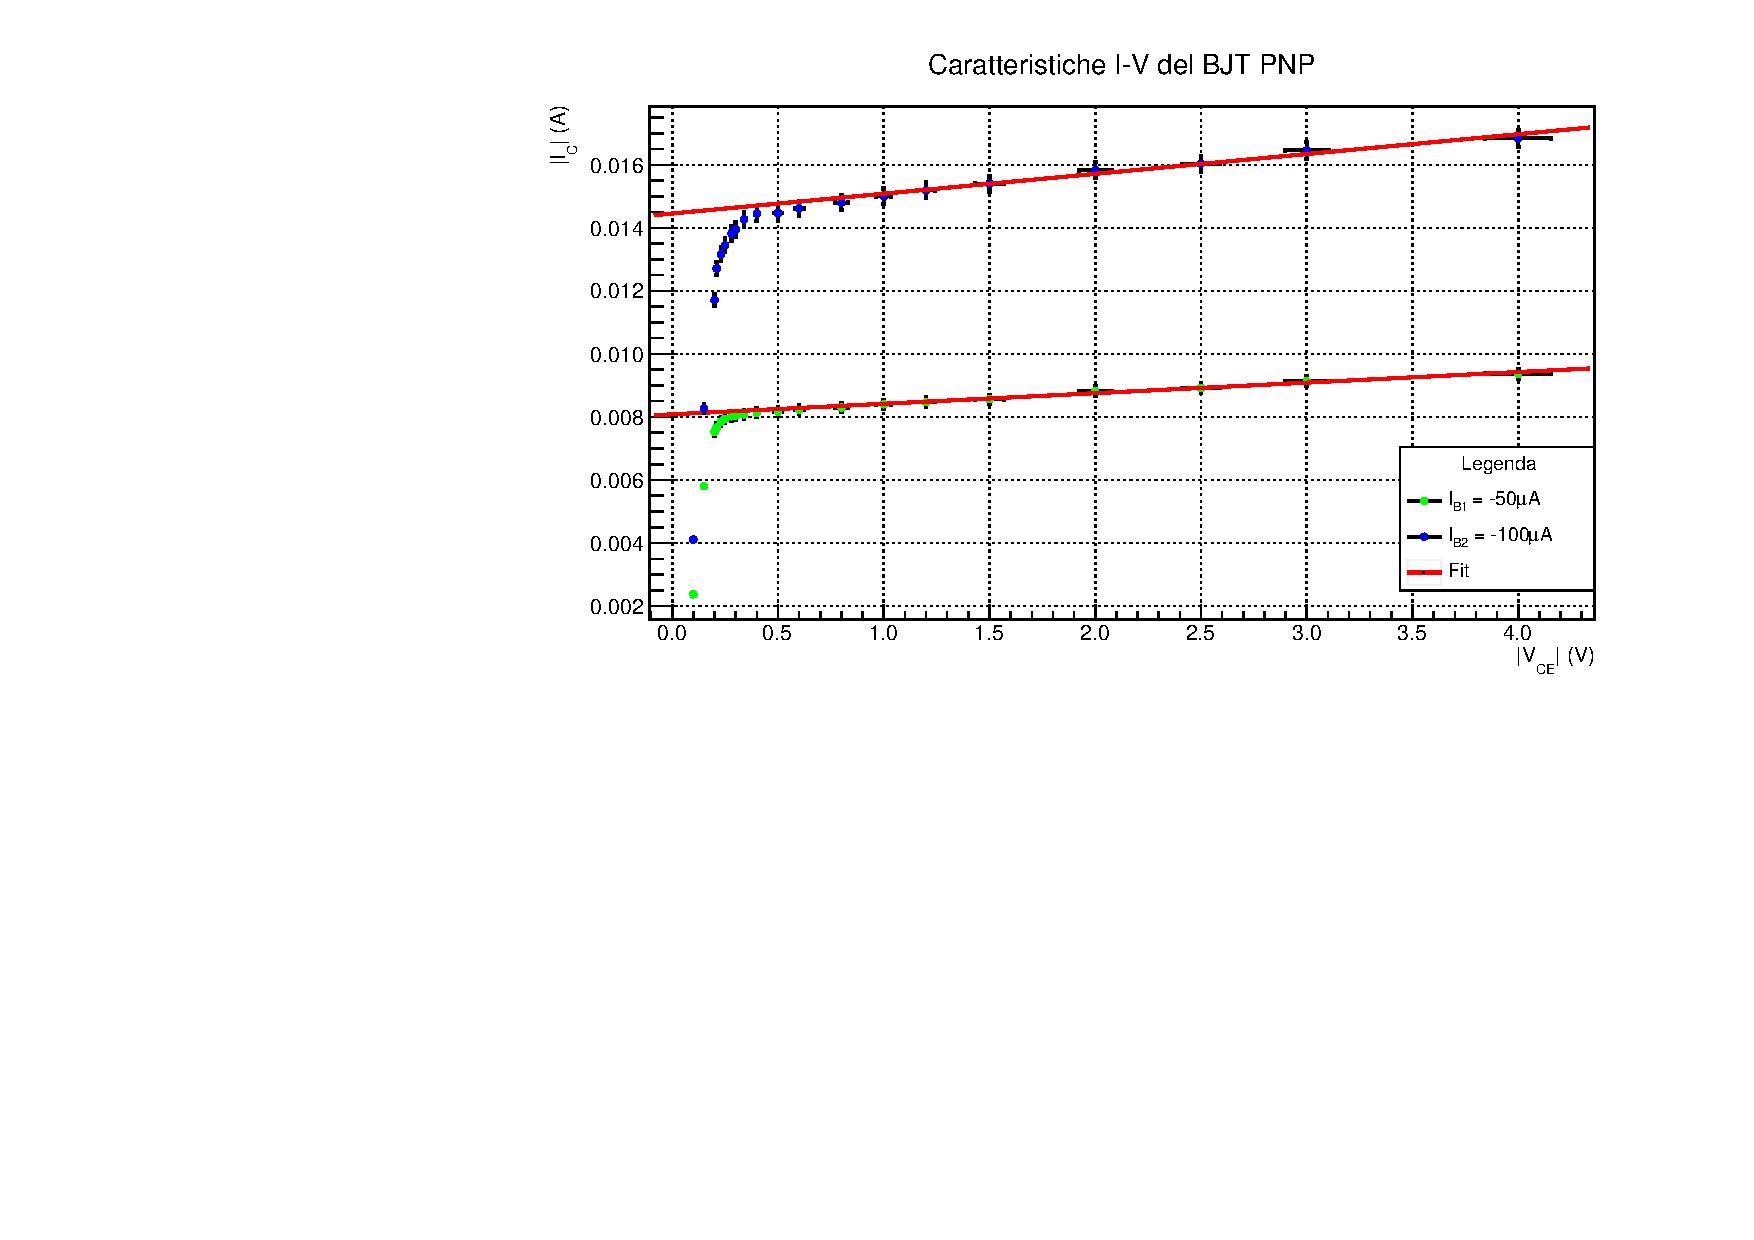
\includegraphics[width=0.9\textwidth]{image/fit.pdf}
    \caption{Grafico con relativi fit delle  caratteristiche $I_C$-$V_{CE}$. In verde riportiamo i dati relativi a $I_{B_1}$, mentre in blu quelli relativi a $I_{B_2}$. Per entrambi i casi il fit è stato svolto per valori della tensione $|V_{CE}|>1$ \si{V}.}
    \label{fig:fit}
\end{figure}

Con i dati riportati in \autoref{tab:data}, presente in \autoref{ch:data}, è stato possibile graficare gli andamenti $I_C$-$V_{CE}$ del transistor per le due correnti di base fissate $I_{B_1}$ e $I_{B_2}$. Per il calcolo delle incertezze sulle varie misure rimandiamo all’\autoref{ch:err}. Con le caratteristiche $I_C$-$V_{CE}$ del transistor è stato possibile effettuare un fit lineare pesato, secondo l'\autoref{eq:fit}, nella regione attiva per ciascun valore di $I_B$, come riportato in \autoref{fig:fit}.

Dopo aver estrapolato dai fit i valori di a e b per entrambe le caratteristiche, abbiamo ricavato la conduttanza $g$ e il guadagno $\beta$ a partire dalle relazioni \eqref{eq:conduttanza} e \eqref{eq:guadagno}. In particolare, per calcolare $\beta$ abbiamo fissato $V_{CE} = -1.0$ \si{V} come tensione di riferimento. Anche in questo caso, per il calcolo delle incertezze su $g$ e $\beta$ rimandiamo all’\autoref{ch:err}.  
Riportiamo i valori dei parametri trovati per le due differenti caratteristiche in \autoref{tab:fit_res}.

\begin{table}[htb]
    \centering
    \begin{tabular}{||c||c||c||}
    \hline \hline
    \multicolumn{3}{||c||}{\textsc{risultati dei fit}}\\
    \hline \hline
      & $I_{B_1} = -50$ \si{\micro\ampere} & $I_{B_1} = -100$ \si{\micro\ampere}\\
    \hline \hline
    $V_a$ & $(24 \pm 5)$ \si{V} & $(23 \pm 4)$ \si{V}\\
    $R_L$ & $(3.0 \pm 0.5)$ \si{\kilo\ohm} & $(1.6\pm 0.3)$ \si{\kilo\ohm} \\
    $g$ & $(0.33 \pm 0.06)$ \si{mS} & $(0.63 \pm 0.12)$ \si{mS} \\
    \hline
    $\beta$ & \multicolumn{2}{c||}{$(1.3 \pm 1.1) \cdot 10^{2}$} \\
    \hline\hline
    \end{tabular}
    \caption{Risultati dei fit con relativi valori della conduttanza $g$ e guadagno $\beta$.}
    \label{tab:fit_res}
\end{table}